\section{Gestion de projet}
    \subsection{Réalisation d’un état des lieux du projet}

Afin de comprendre les sources du projet \COREL et le travail effectué lors des projets précédents, il a été nécessaire de faire un état des lieux, à intégrer dans le cahier des charges.\footnote{Voir l'annexe A} En effet, les projets \LSC et \EPJ n'ont pas produit de documentation, ce qui rend la compréhension de ces projets difficile. Seuls les chercheurs ayant travaillé sur ces projets sont à même d'expliquer le travail effectué et les productions qui en découlent. De plus, sans connaissances préalables sur le droit chinois, les sources numériques produites ne sont pas suffisamment claires pour être instantanément comprises par un ingénieur et ne se suffisent pas à elles-mêmes, d'autant plus avec un schéma d'encodage personnalisé, qui a pu se transformer avec le temps. Dès lors, l'état des lieux des projets précédents est indispensable afin de préparer les données pour le projet \COREL, d'autant plus que l'enrichissement des données \LSC et \EPJ est toujours en cours. 

En l'absence de documentation rédigée pendant le projet, ou de documents de travail détaillant les étapes de traitement des données effectuées, l'état des lieux fournit une description des sources numériques au début du projet \COREL. Puisque les sources \XML ont été transformées en \TEI pendant le stage, l'état des lieux n'est pas exhaustif sur le schéma d'encodage personnalisé du site \LSC mais fournit un aperçu de la transformation \XSLT et des raisons pour lesquelles le schéma \LSC ne convenait plus. Cette partie du cahier des charges vise à donner un premier aperçu des documents pour en comprendre la composition générale. 

Les productions du projet \EPJ sont, quant à elles, multiples et ont demandé une description plus approfondie. Appréhender ces données est un travail complexe, puisque les formats des données sont hétérogènes, même au sein du projet \EPJ. De plus, le travail étant effectué par un prestataire, l'équipe du projet n'a pas de visibilité sur les différentes étapes de travail effectuées pour aboutir à ces formats de données. L'état des lieux rédigé dans le cahier des charges reste donc une description des données fournies par le prestataire et du travail effectué par les chercheurs, mais ne peut détailler de manière exhaustive toutes les étapes de la chaîne de traitement.

L'état des lieux est organisé selon le type de données : les annotations, les métadonnées et les liens entre les lois. Ces trois types de données ne correspondent pas nécessairement à un seul format, c'est pourquoi organiser l'état des lieux un format après l'autre n'est pas pertinent et complexifie la compréhension. Les annotations, par exemple, sont accessibles au format \JSON, \csv ou \tsv et directement via le visualiseur Mirador. Ce travail de description s'accompagne parfois de modélisations \UML pour faciliter la compréhension. En effet, le recensement de tous les liens entre les lois est un fichier assez dense et complexe et qui ne possède pas de documentation. Seuls les chercheurs du projet \EPJ sont capables d'utiliser ce recensement comme outil de travail. Or, retracer la généalogie des lois est l'un des axes majeurs du projet, ce document est donc essentiel afin de réaliser le projet. Cet exemple permet de souligner l'importance de fournir une documentation et des documents de travail clairs. En effet, deux modélisations suffisent pour expliciter ce document et permettent de comprendre facilement quels types de liens sont possibles entre les lois. L'établissement d'un cahier des charges et la production d'une documentation pendant le stage sont donc essentiels pour la suite du projet.  

\begin{figure}
    \centering
    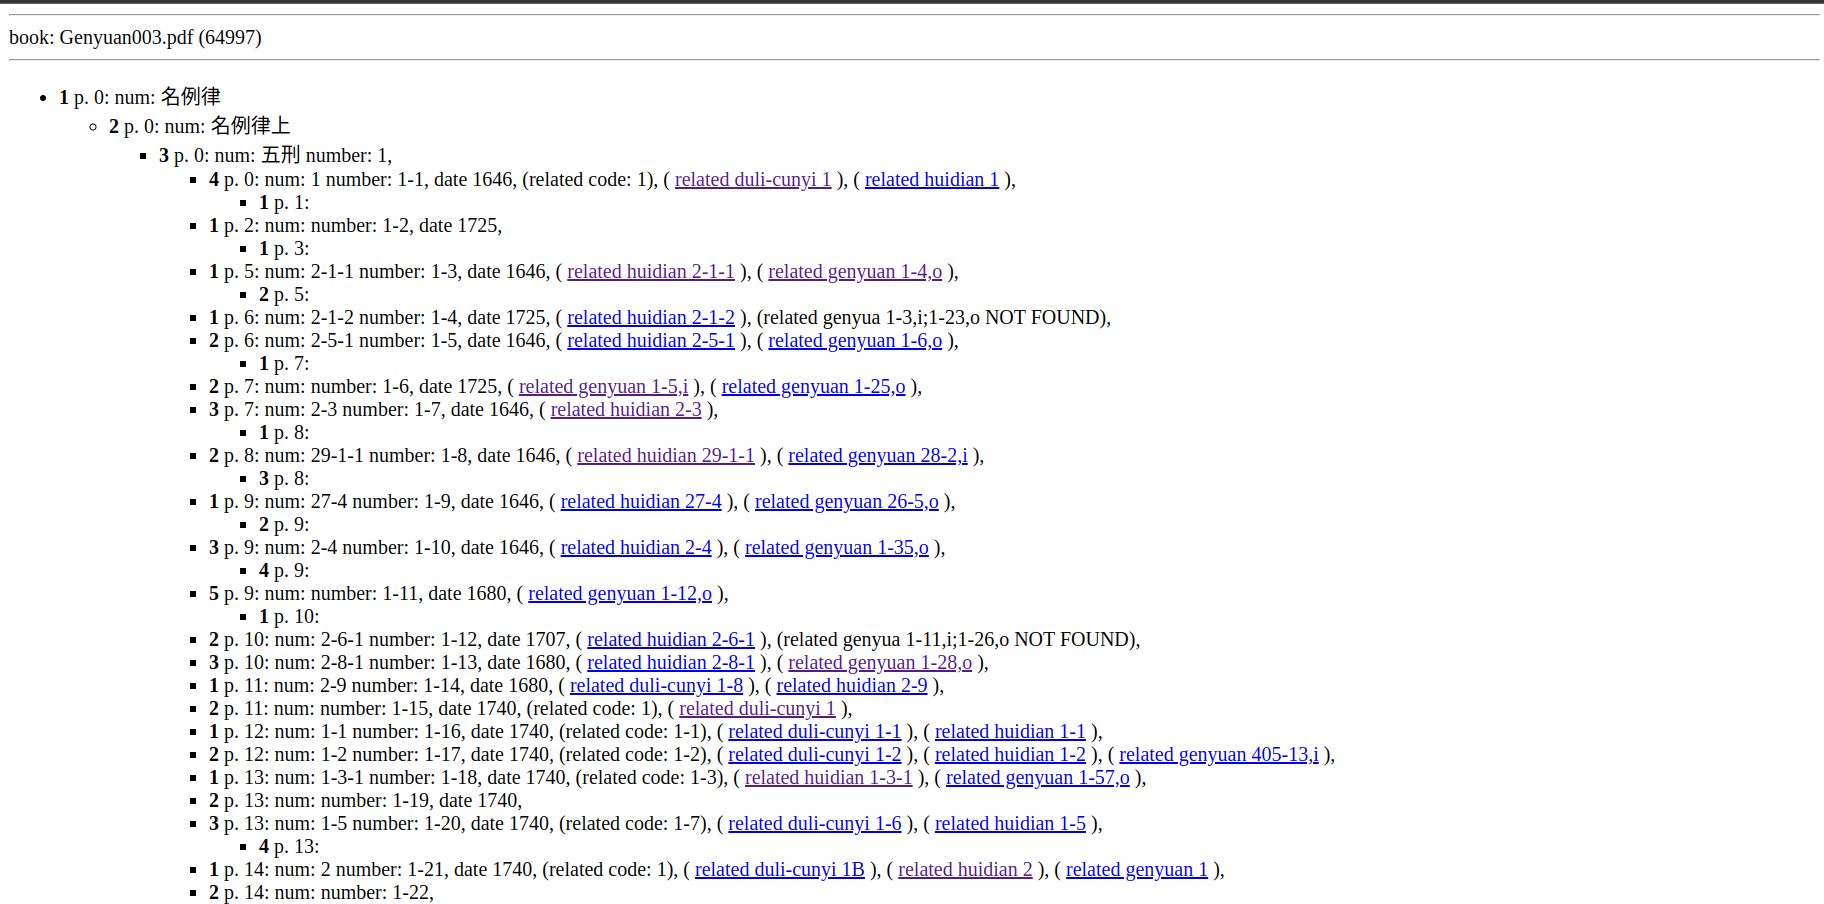
\includegraphics[width=\textwidth]{images/image6.png}
    \caption{Capture d'écran du fichier de recensement des liens entre les lois.}
\end{figure}

\subsection{Définir les livrables attendus du projet}

L'établissement d'un cahier des charges fonctionnel permet également de définir clairement les livrables attendus. Le projet \COREL n'avait jusqu'alors pas de descriptif précis des livrables attendus en fin de projet. Lors de la candidature à l'appel à projets pour le financement \CollEx Persée, les chercheurs ont défini comme livrable un \POC sur trois lois représentatives du corpus pour créer un \cv. Toutefois, ce livrable est considéré par l'équipe du projet comme un engagement minimal, et le périmètre du projet est en réalité plus large. 

Une grande partie du stage a donc été consacrée à définir ce périmètre, en assurant la cohésion entre le projet de recherche et sa réalisation technique, en prenant en considération la volonté des chercheurs d'élargir leur champ de compétences en participant à certains aspects numériques du projet, comme l'encodage par exemple. Il a donc fallu dans un premier temps rassembler les idées de chaque membre de l'équipe lors de réunions, tout en gardant à l'esprit le besoin d'utiliser des outils et méthodes accessibles aux chercheurs, c'est-à-dire sans pré-requis techniques. Lors des réunions de conception du projet, il s'est avéré que les chercheurs souhaitaient un livrable bien plus étendu que le \POC : une édition en ligne la plus exhaustive possible (ajout de commentaires, entités nommées...), la reconstitution de la législation entre 1644 et 1911 et également des visualisations interactives pour retracer la généalogie d'une loi. Ces livrables n'avaient toutefois pas été clairement définis car il était important pour l'équipe de rester flexible durant toute la durée du projet. Toutefois, cette manière d'envisager le projet présente un risque conséquent. En effet, sans livrable défini ni périmètre, le projet peut ne pas être réalisé dans le temps imparti du financement et laissé à l'abandon comme c'est le cas du site web \LSC. Le cahier des charges fonctionnels a ainsi permis aux chercheurs d'exprimer toutes leurs attentes et de fixer clairement le périmètre, en dialogue avec l'ingénieur du projet. 

\subsection{Prioriser certains aspects du projet}

Ce travail de définition des besoins et des livrables en sortie du projet ne signifie pas pour autant que le projet manque de flexibilité et lors des réunions, il est clairement apparu que les besoins du projet étaient hiérarchisés. En effet, une édition en ligne simple et la reconstitution de la législation sont les deux éléments les plus importants pour assurer la bonne réalisation du projet. Toutefois, le cahier des charges ne se limite pas à ces deux aspects du projet afin d'englober à la fois les besoins secondaires comme le balisage des entités nommées ou les visualisations, mais aussi les perspectives d'enrichissement futures. Trois niveaux du livrable final ont donc ainsi été définis : en premier lieu, tous les besoins hors périmètre ont été écartés du projet. Cela concerne les données dont le projet ne dispose pas, notamment les recueils de cas qui sont actuellement en cours de numérisation par la bibliothèque d'études chinoises. Ces données sont intéressantes du point de vue scientifique et apportent une plus-value aux textes de lois, mais ne sont pas indispensables dans le cadre du projet. Elles feront l'objet d'un autre projet ou seront ajoutées après l'échéance du financement. 

Il a ensuite fallu déterminer quelles données étaient primordiales pour la réalisation de l'édition en ligne et le \cv, et lesquelles seraient intéressantes à ajouter si le temps le permet. Le site \LSC permet de démontrer que les données en l'état sont suffisantes pour publier une édition en ligne. Toutefois, les données nécessaires au \cv ne figurent que dans les annotations et ne sont pas exhaustives. La priorité est donc d'ajouter ces données manquantes dans l'encodage \TEI, notamment les dates de validité de chaque loi et des identifiants uniques permettant de les lier aux annotations. Les ajouts de commentaires ou d'entités nommées, quant à eux, sont des éléments secondaires, mais qui font partie du périmètre car ils concernent les textes de lois déjà édités, et qu'une partie de ces données a déjà été balisée dans le \XML. 

Déterminer clairement les livrables attendus en priorisant certains aspects du projet a ainsi permis de lancer la phase de préparation des données. 

 \section{Importance de l’étape de préparation des données}
    \subsection{La diversité des données des projets précédents}

Une fois les données essentielles identifiées, il est possible de commencer à préparer les données. Cette étape est primordiale afin de réaliser le projet. 

\subsection{Établissement d’un écosystème de données}

§ Paragraphe 1

Idée :\\
Exemple :\\
Référence :\\
Transition :\\

§ Paragraphe 2

Idée :\\
Exemple :\\
Référence :\\
Transition :\\

§ Paragraphe 3

Idée :\\
Exemple :\\
Référence :\\
Transition :\\

